\chapter{Spectrometric chain PCB integration}
The only way to improve the performances of the spectrometric chain is to integrate it into a small PCB - short the signal routes, reduce parasitic capacitances at preamplifier input and improve the shielding. The various prototypes were designed as 2-side PCBs and manufactured by using the special milling machine to remove cooper from cuprextit plates. The PCB consisting mainly of smd parts was then assembled by manual soldering.

\section{Scheme and Layout}
The main parts of spectrometric chain integrated PCB are: photodiode input connector, preamplifier, second stage amplifier, shaper module, output buffer optimized for 50\nobreakspace$\Omega$ transmission line, bipolar voltage supply for modules and bias voltage supply for photodiode. To surround the sensitive parts with sufficient shielding, the PCB is placed into aluminium box with drilled photodiode window. The functional scheme can be seen on fig. \ref{schematic} and the real layout for PCB can be seen on figs. \ref{layout top} and \ref{layout bottom}.



\begin{figure}[H]
 \centering
 
\includegraphics[scale=0.35, angle = 0]{./pictures/NoPicture.jpg}
 \caption{PCB in aluminium box.}
 \label{PCBbox}
 
\end{figure}


\begin{figure}[H]
 \centering
 
\includegraphics[scale=0.35, angle = 0]{./pictures/NoPicture.jpg}
 \caption{Fully assembled PCB with attached cremat modules.}
 \label{PCBphyss}
 
\end{figure}



\newpage

\begin{figure}[H]
 \centering
 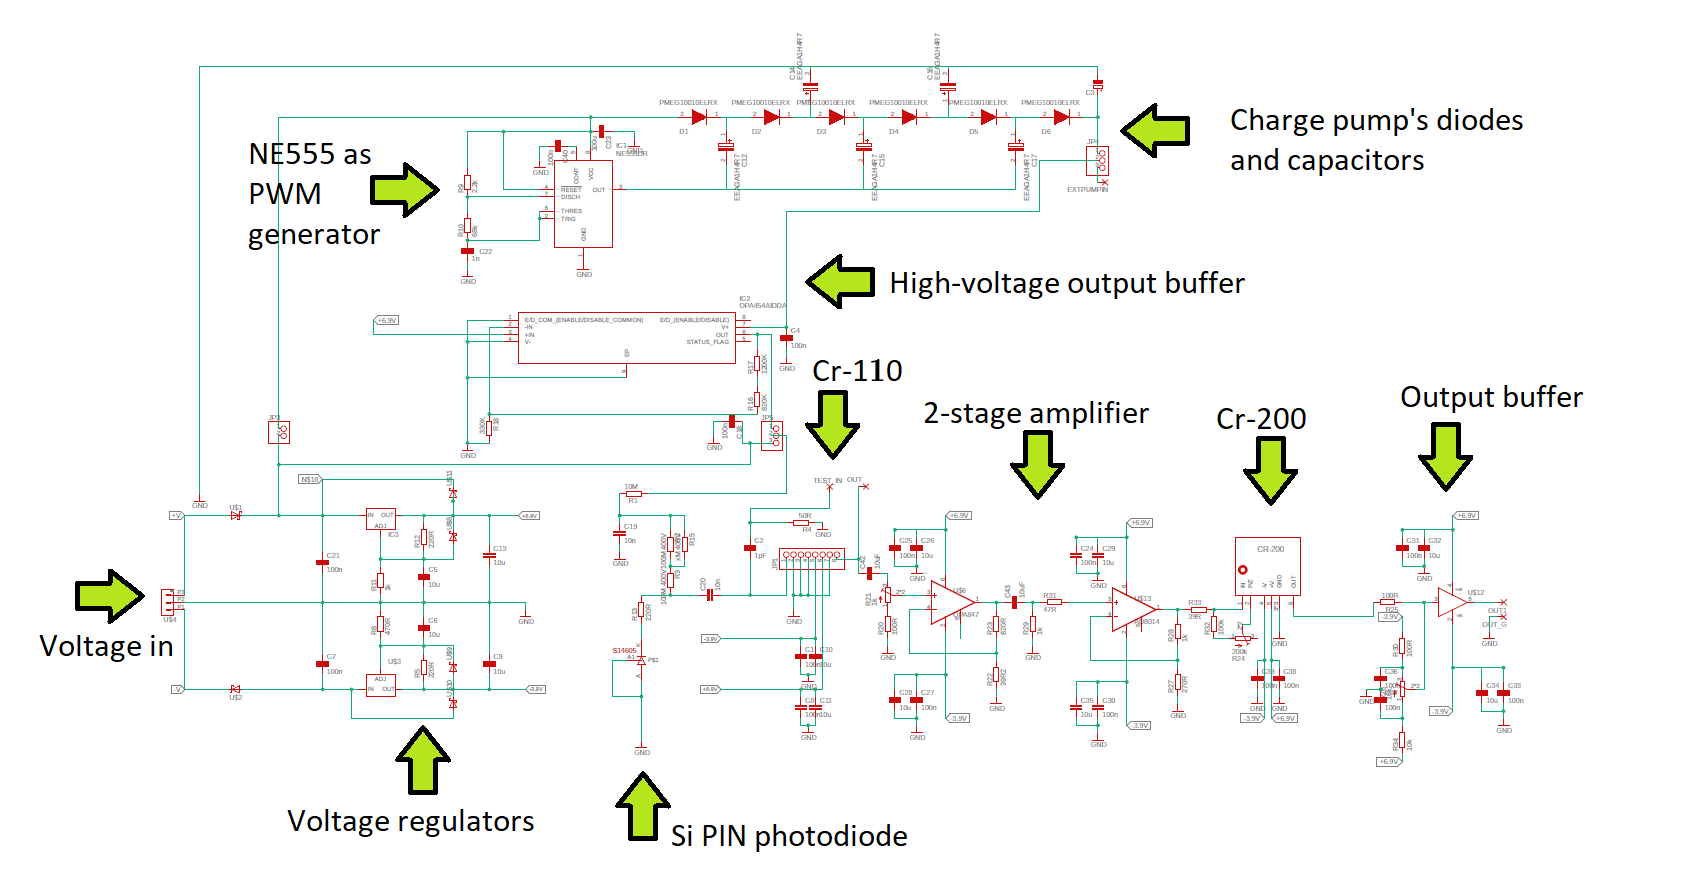
\includegraphics[scale=0.5, angle = 90]{./pictures/schemaPopis.png}
 \caption{Schematic of spectrometric chain PCB designed in EAGLE \cite{eagle}. Full schematic can be found in attachments.}
 \label{schematic}
 
\end{figure}

\newpage

\begin{figure}[H]
 \centering
 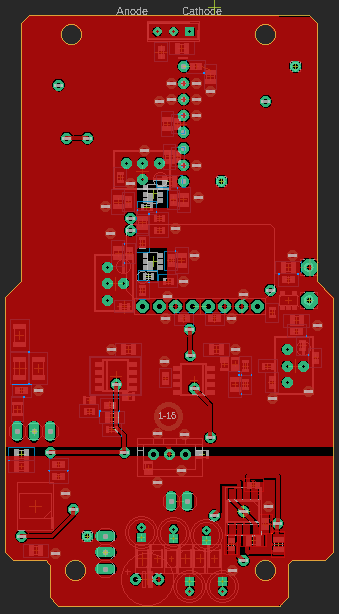
\includegraphics[scale=0.8, angle = 90]{./pictures/S14topLay.png}
 \caption{Layout of spectrometric chain PCB designed in EAGLE \cite{eagle}, top side layer.}
 \label{layout top}
 
\end{figure}

\begin{figure}[H]
 \centering
 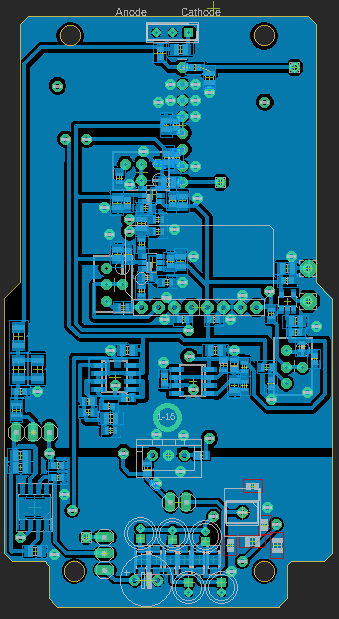
\includegraphics[scale=0.8, angle = 90]{./pictures/S14bottomLay.png}
 \caption{Layout of spectrometric chain PCB designed in EAGLE \cite{eagle}, bottom side layer.}
 \label{layout bottom}
 
\end{figure}
\newpage





\section{Grounding and Shielding}
To allow all the currents to have their return path with a sufficient conductivity, the main GND signal has to be spilled all around the circuit board. Even a small resistances in these paths may cause additional noises in signals. Currents from non-signal parts such as charge pump should have their return path different from the path of signal parts, and thus the spilled GND has to be cut to several separate parts connected together only at input voltage connector.

\par
The shielding box has to be connected to GND in carefully selected place to prevent the induced currents from shielding to flow over the signal ground of the detector. The best place to connect the shielding box with GND is near the input voltage connector.


\section{Photodiode input and preamplifier}
The photodiode is situated inside the box, and the cathode is connected to bias voltage and to preamplifier (Cr-110) by capacitive coupling (10 nF capacitor). Cr-110 application note also mentions an optional 220 $\Omega$ resistor connected before coupling capacitor to prevent Cr-110 breakdown by large current spikes. Our experiences show that this resistor should not be omitted.

\par
The signal route has to be as short as possible. The layout should also be designed in ways to reduce the parasitic capacitances at the preamplifier input - the cooper connected to ground (GND) should be removed from areas around the signal input route and around input bias voltage route. 

\section{Amplification}
The preamplifier output is routed over capacitive coupling (to eliminate unwanted offset) and over potentiometer divider (to adjust signal strength) to the amplification stages. 

First amplification is achieved by two non-invering amplifiers made of OPA847 opamps. Each stage has the amplification of 32$\times$ (or less, this is different for every of our prototypes). Additional amplification 10$\times$ is done by shaper module Cr-220. The experiences show that the fast opamps are inclinable to unwanted oscillacions, and thus the GND has to be removed around the opamp from both sides of PCB. The output of shaper module is routed directly to output buffer opamp MAXnumber. The end of chain is the buffer's output connected to the SMA connector mounted onto the aluminium box.

\par



\section{Voltage supply}
The regulation of input voltages (usually +15 V and -15 V) is done by LM317 and LM337 regulators, which convert input supply voltages into +7 V and -4 V. The output voltage of regulators is set by two resistors. However, these regulators produce heat, which negatively affects the SNR, so this heat has to be taken out of the circuit board by the thermal bridge connection to the aluminium box. To stabilize the temperature during the long runs, the shielding case has two additional peltier couples with fan attached onto it.

\par
S14605 requires bias voltage around +50 V, which can be supplied by 3-stage charge pump, assembled simply from capacitors, diodes and PWM generator - for example NE555. The charge pump multiplies the input voltage +15 V to +60 V. However, the charge pump is not a stiff voltage source - even a low output current can cause a large dropout, so the real bias voltage is around +50 V. The pump's output has to be filtered, because it can contain voltage spikes from PWM (NE555's frequency is set to 10 kHz). To filter this high voltage output the high-voltage opamp OPA454 is connected as buffer - the pump's voltage is connected as opamp supply, and the voltage from regulator (+7 V) is connected into opamp negative input pin. There is also a jumper which allows to switch between +15 V (for BPW34 photodiode) and +50 V.

\section{}



\section{}


